\pdfminorversion=4
\documentclass[aspectratio=169]{beamer}

\mode<presentation>
{
  \usetheme{default}
  \usecolortheme{default}
  \usefonttheme{default}
  \setbeamertemplate{navigation symbols}{}
  \setbeamertemplate{caption}[numbered]
  \setbeamertemplate{footline}[frame number]  % or "page number"
  \setbeamercolor{frametitle}{fg=white}
  \setbeamercolor{footline}{fg=black}
} 

\usepackage[english]{babel}
\usepackage{inputenc}
\usepackage{tikz}
\usepackage{courier}
\usepackage{array}
\usepackage{bold-extra}
\usepackage{minted}
\usepackage[thicklines]{cancel}
\usepackage{fancyvrb}

\xdefinecolor{dianablue}{rgb}{0.18,0.24,0.31}
\xdefinecolor{darkblue}{rgb}{0.1,0.1,0.7}
\xdefinecolor{darkgreen}{rgb}{0,0.5,0}
\xdefinecolor{darkgrey}{rgb}{0.35,0.35,0.35}
\xdefinecolor{darkorange}{rgb}{0.8,0.5,0}
\xdefinecolor{darkred}{rgb}{0.7,0,0}
\definecolor{darkgreen}{rgb}{0,0.6,0}
\definecolor{mauve}{rgb}{0.58,0,0.82}

\title[2023-10-25-tiled-uproot-irishep-topical]{Tiled-Uproot: a use of Awkward Arrays in Tiled \\ and a possible Tiled Adapter}
\author{Jim Pivarski}
\institute{Princeton University -- IRIS-HEP}
\date{October 25, 2023}

\usetikzlibrary{shapes.callouts}

\begin{document}

\logo{\pgfputat{\pgfxy(0.11, 7.4)}{\pgfbox[right,base]{\tikz{\filldraw[fill=dianablue, draw=none] (0 cm, 0 cm) rectangle (50 cm, 1 cm);}\mbox{\hspace{-8 cm}
\includegraphics[height=1 cm]{princeton-logo-long.png}\hspace{0.1 cm}\raisebox{0.1 cm}{
\includegraphics[height=0.8 cm]{iris-hep-logo-long.png}}\hspace{0.1 cm}}}}}

\begin{frame}
  \titlepage
\end{frame}

\logo{\pgfputat{\pgfxy(0.11, 7.4)}{\pgfbox[right,base]{\tikz{\filldraw[fill=dianablue, draw=none] (0 cm, 0 cm) rectangle (50 cm, 1 cm);}\mbox{\hspace{-8 cm}
\includegraphics[height=1 cm]{princeton-logo.png}\hspace{0.1 cm}\raisebox{0.1 cm}{
\includegraphics[height=0.8 cm]{iris-hep-logo.png}}\hspace{0.1 cm}}}}}

% Uncomment these lines for an automatically generated outline.
%\begin{frame}{Outline}
%  \tableofcontents
%\end{frame}

% START START START START START START START START START START START START START

\begin{frame}{Finding data in a ROOT file involves several round-trips}
\vspace{1 cm}
\only<1>{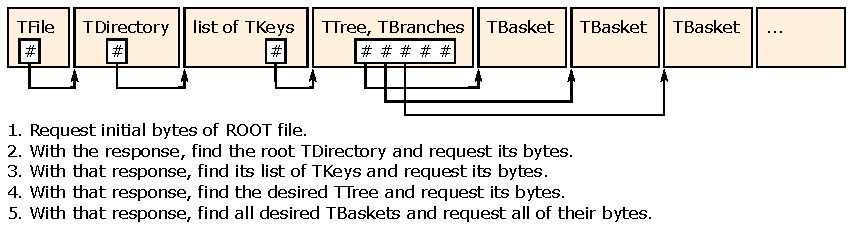
\includegraphics[width=\linewidth]{finding-seek-positions.pdf}}\only<2->{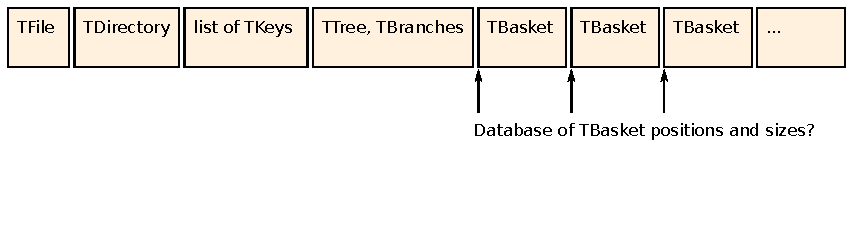
\includegraphics[width=\linewidth]{finding-seek-positions-2.pdf}}

\begin{uncoverenv}<3->
\vspace{-1.25 cm}
{\large Why would you want to do that?}

\vspace{0.25 cm}
\begin{itemize}
\item Replace the latency of 4~round trips with the latency of a (nearby) database.
\item Specialized TTree/RNTuple access for large sets of files.
\item Leave a set of ROOT files in place, so they don't need to be converted and can be accessed in traditional ways as well.
\item Can be made to look the same as a database of user-contributed Awkward Arrays.
\end{itemize}
\end{uncoverenv}
\end{frame}

\begin{frame}{Nick Smith's columnservice prototype}
\vspace{0.5 cm}

\begin{columns}
\column{0.3\linewidth}
\vspace{-0.5 cm}
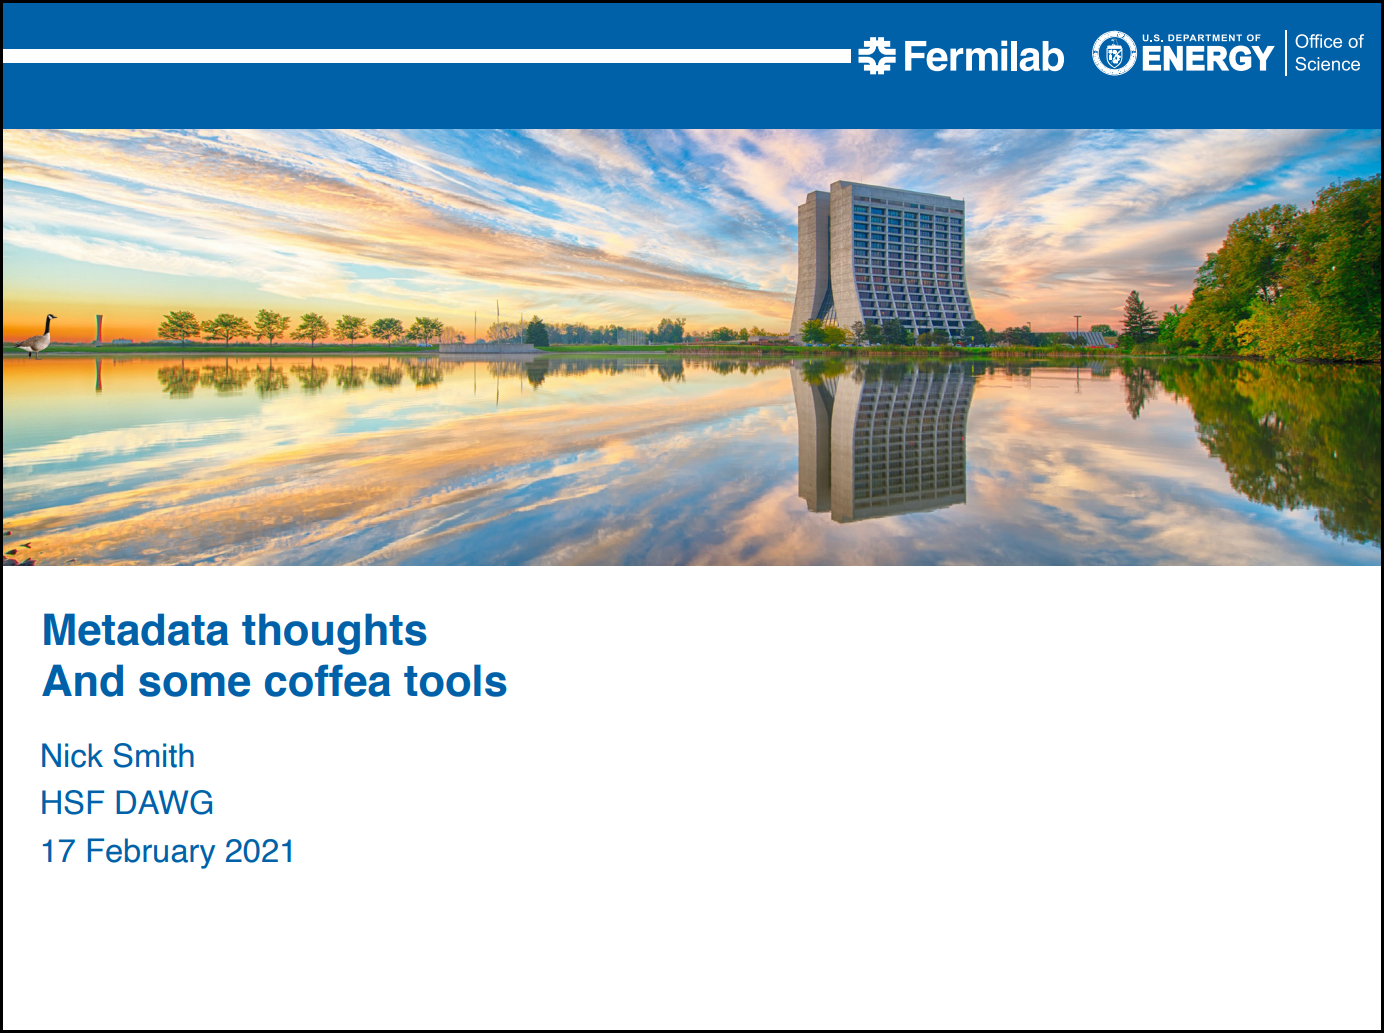
\includegraphics[width=\linewidth]{nsmith-1.png}

\vspace{0.5 cm}
\textcolor{blue}{\bf\url{https://github.com/CoffeaTeam/columnservice}}

\vspace{0.5 cm}
\textcolor{gray}{(last activity: Mar 2021)}

\column{0.7\linewidth}
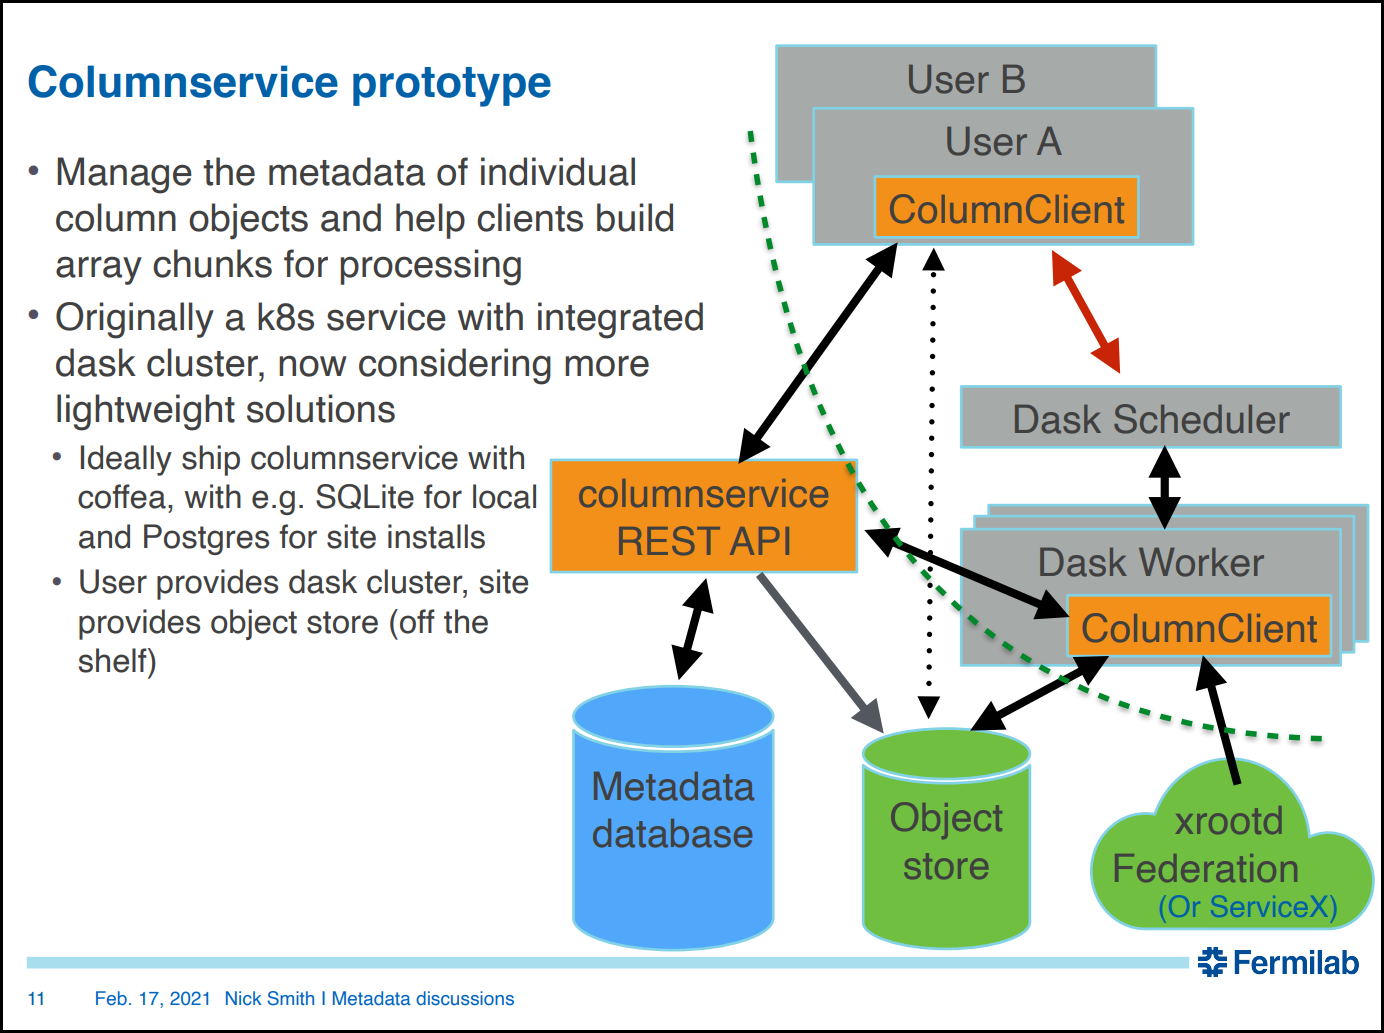
\includegraphics[width=\linewidth]{nsmith-2.png}
\end{columns}
\end{frame}

\begin{frame}{Nick Smith's columnservice prototype}
\vspace{0.35 cm}
\begin{center}
\only<1>{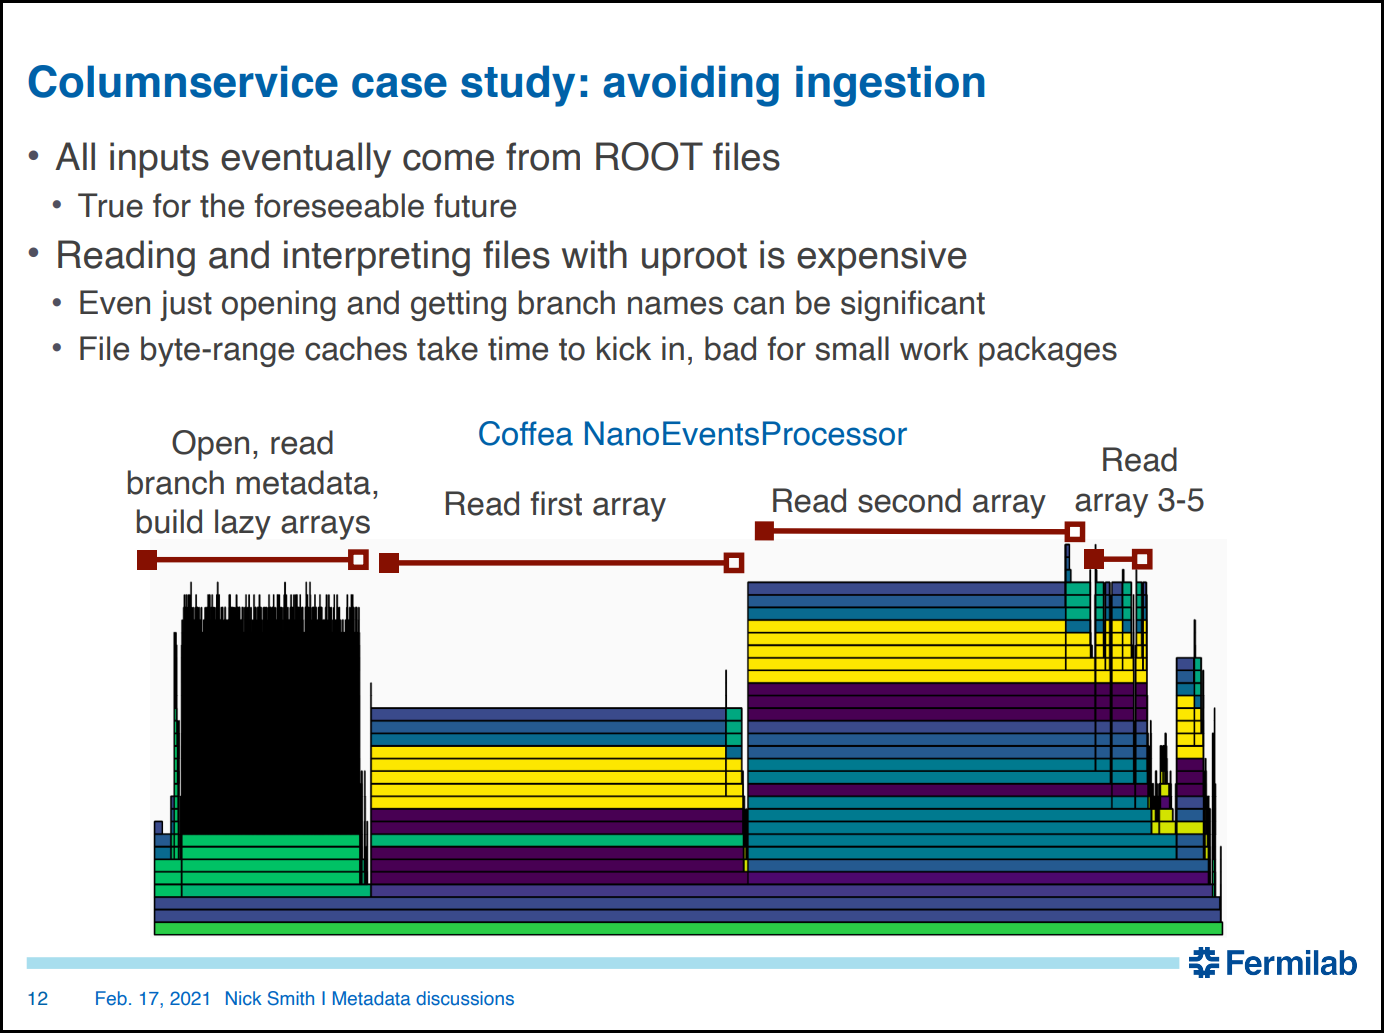
\includegraphics[width=0.7\linewidth]{nsmith-3.png}}\only<2>{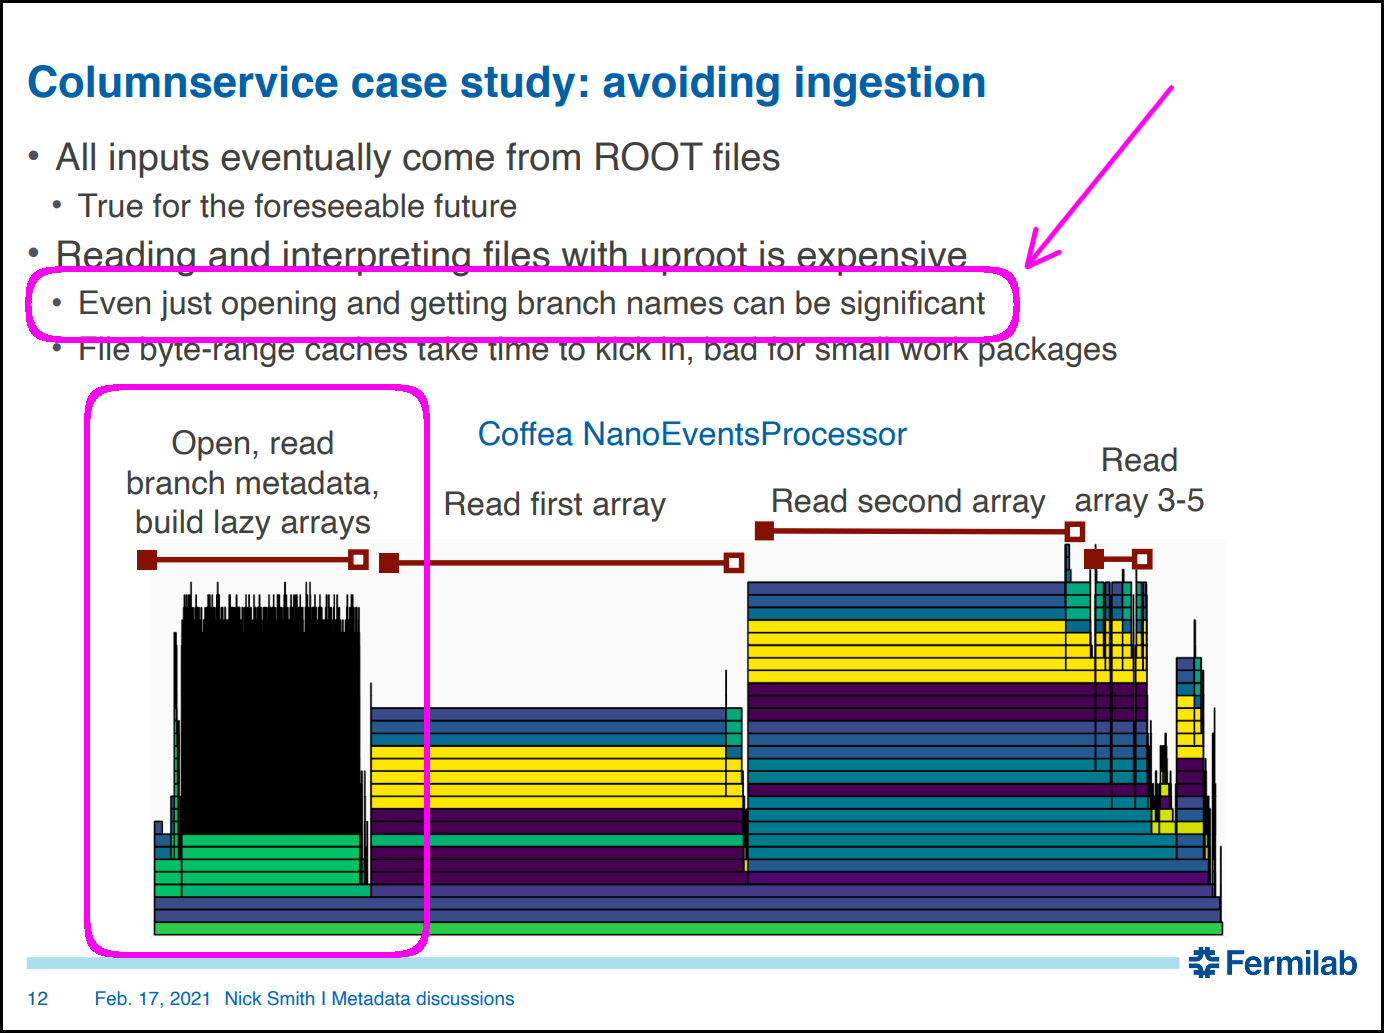
\includegraphics[width=0.7\linewidth]{nsmith-3-5.png}}
\end{center}
\end{frame}

\begin{frame}{ROOT metadata is Awkward: large and complex structured}
\vspace{0.5 cm}

\underline{Typical ROOT file (CMS NanoAOD, DoubleMuon)}:

\vspace{0.2 cm}
\begin{itemize}
\item 2.343~GB (13~GB uncompressed)
\item 1405 TBranches; 413 for non-triggers \textcolor{gray}{(29\%)}
\item 594\,364 TBaskets; 252\,496 for non-triggers \textcolor{gray}{(42\%)}
\item 2.338~GB TBasket data; 3.6~kB/basket for triggers, 9.2 for non-triggers \textcolor{gray}{(88\%)}
\end{itemize}

\vspace{0.35 cm}
\uncover<2->{$\longrightarrow$ 14.7~MB as Awkward metadata; 4.9~MB gzip-compressed \textcolor{gray}{(ROOT uses 5.1~MB)}}

\vspace{0.35 cm}
\uncover<3->{$\longrightarrow$ uncompressed metadata is 0.6\% as large as the data itself}

\vspace{0.35 cm}
\uncover<4->{$\longrightarrow$ 6.7~TB dataset (2040~files) requires 41~GB of metadata in the database}
\end{frame}

\begin{frame}[fragile]{ROOT metadata is Awkward: large and complex structured}
\vspace{0.3 cm}

\underline{Metadata as an Awkward Array (showing its type)}:

\vspace{-0.1 cm}
\scriptsize
\begin{columns}
\column{0.5\linewidth}
\begin{minted}{javascript}
1 * {
    offsets: var * int64,
    era: var * {
        treename: string,
        names: var * string,
        interpretations: var * bytes   // pickle
    },
    prefix: var * string,
    file: var * {
        filename: string,
        tree: {
            run: var * {
                seek: int64,   // must be int64
                stop: int64,   // could be int32
                bytes: int64   // could be int32
            },
            luminosityBlock: var * {
                seek: int64,
                stop: int64,
                bytes: int64
            },
\end{minted}

\column{0.5\linewidth}
\begin{minted}{javascript}
            event: var * {
                seek: int64,
                stop: int64,
                bytes: int64
            },
            CaloMET_phi: var * {
                seek: int64,
                stop: int64,
                bytes: int64
            },
            CaloMET_pt: var * {
                seek: int64,
                stop: int64,
                bytes: int64
            },
            ...        // 1405 TBranches
        },
        era: int64,    // lookup era
        prefix: int64  // lookup prefix
    }
}
\end{minted}
\end{columns}

\end{frame}

\begin{frame}{Why is this structure useful?}
\large
\vspace{0.5 cm}

\begin{itemize}\setlength{\itemsep}{0.5 cm}
\item Global \mintinline{javascript}{offsets} to lookup files for a given range of entries.
\item Small number of \mintinline{javascript}{era}s allows \mintinline{javascript}{treename}, TBranch \mintinline{javascript}{names}, and (pickled) \mintinline{javascript}{interpretations} to vary in the dataset (e.g. new trigger lines).
\item \mintinline{javascript}{prefix} for \mintinline{javascript}{filename} avoids duplicated characters in long path URLs.
\item Separate records for each TBranch allows TBranches to be queried independently. (TBranches that aren't in all files have \mintinline{javascript}{option} type.)
\item Same number of TBasket \mintinline{javascript}{seek} positions, local entry \mintinline{javascript}{stop} values, and number of \mintinline{javascript}{bytes} share a variable-length list (\mintinline{javascript}{var}).
\end{itemize}
\end{frame}




\end{document}
